\documentclass[12pt, a4paper]{article}
\usepackage{array}
\usepackage{graphicx}
\usepackage{longtable}
\usepackage{etoolbox}
\usepackage{subcaption}
\usepackage{float}
\usepackage{amsmath}
\usepackage{mathtools}
\usepackage[nottoc]{tocbibind}
\usepackage[intoc]{nomencl}

%for clickable table of contents
\usepackage{hyperref}
\hypersetup{
    colorlinks,
    citecolor=black,
    filecolor=black,
    linkcolor=black,
    urlcolor=black
}

%define command for symbol denoting "average of"
\newcommand*\mean[1]{\bar{#1}}

%paragraph spacing and indentation
\setlength{\parindent}{0em}
\setlength{\parskip}{1em}

%counter for numbering the rows of tables
\newcounter{rowcntr}[table]
\renewcommand{\therowcntr}{\thetable.\arabic{rowcntr}}
% A new columntype to apply automatic stepping
\newcolumntype{N}{>{\refstepcounter{rowcntr}\therowcntr}c}
% Reset the rowcntr counter at each new tabular
\AtBeginEnvironment{tabular}{\setcounter{rowcntr}{0}}

\begin{document}

\section{Test list of Tables}
\listoftables

\section{Test Labels}
Testing brown to light label: \ref{row:prop_correct_test_a1p5_hand_brown_to_hand_light}

\section{Test Appendix}
\begin{longtable}{|N||c|c|c|}
	\caption{Test results of proportional brightening with correction for dark spots, $\alpha = 1.5$\label{tab:prop_correct_test_a1p5}}\\
	\hline
	\multicolumn{1}{|c||}{No.} & Original & Target & Results \\ 
	\hline
	    \label{row:prop_correct_test_a1p5_hand_dark_to_hand_brown} &
  \begin{minipage}{.29\textwidth}
    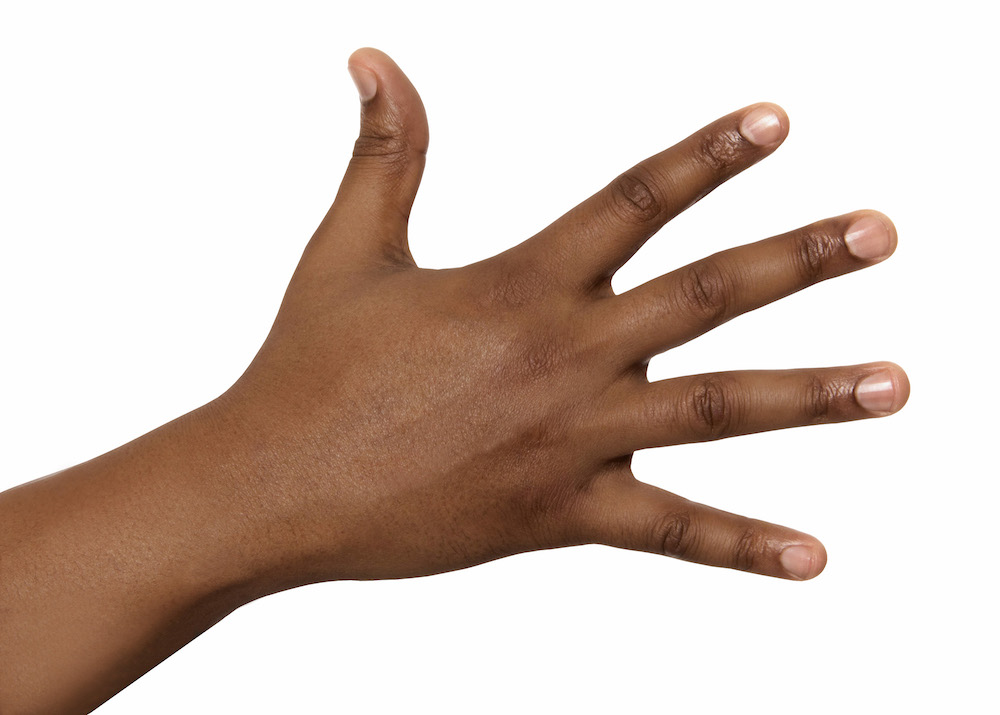
\includegraphics[width=\textwidth,height=\textheight,keepaspectratio]{../inputs/hand_dark.jpg}
  \end{minipage} & 
  \begin{minipage}{.29\textwidth}
    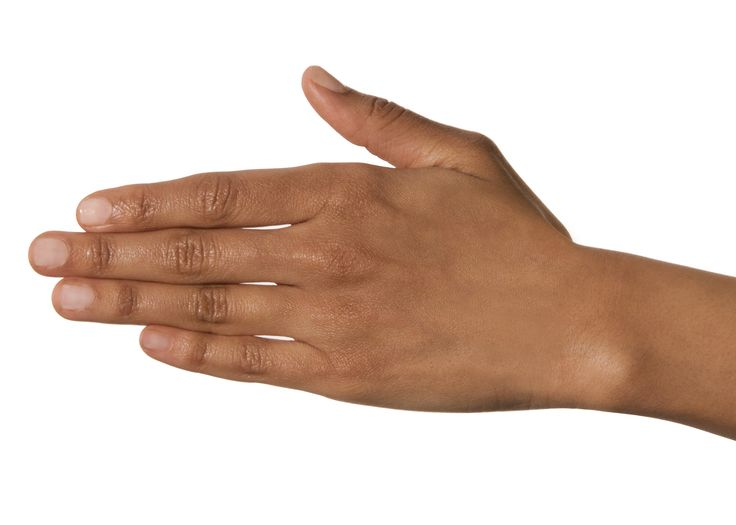
\includegraphics[width=\textwidth,height=\textheight,keepaspectratio]{../inputs/hand_brown.jpg}
  \end{minipage} & 
  \begin{minipage}{.29\textwidth}
    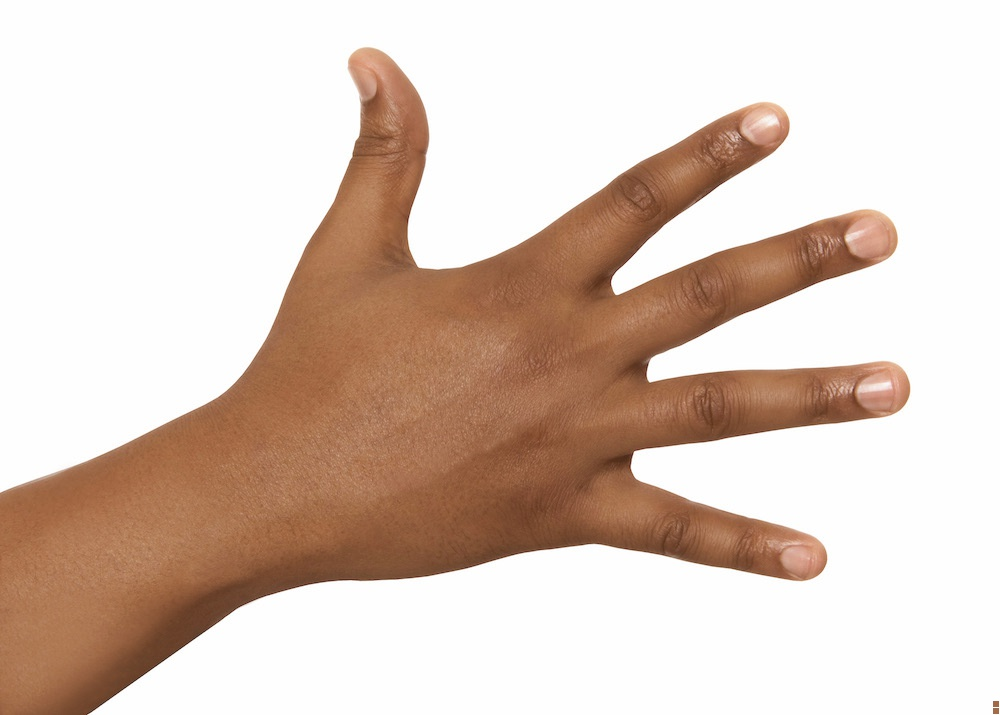
\includegraphics[width=\textwidth,height=\textheight,keepaspectratio]{../rc_test/outputs/20170521_proportional_corrected_test_alpha1p5/hand_dark_to_hand_brown.jpg}
  \end{minipage} \\
\hline  \label{row:prop_correct_test_a1p5_hand_dark_to_hand_light} &
  \begin{minipage}{.29\textwidth}
    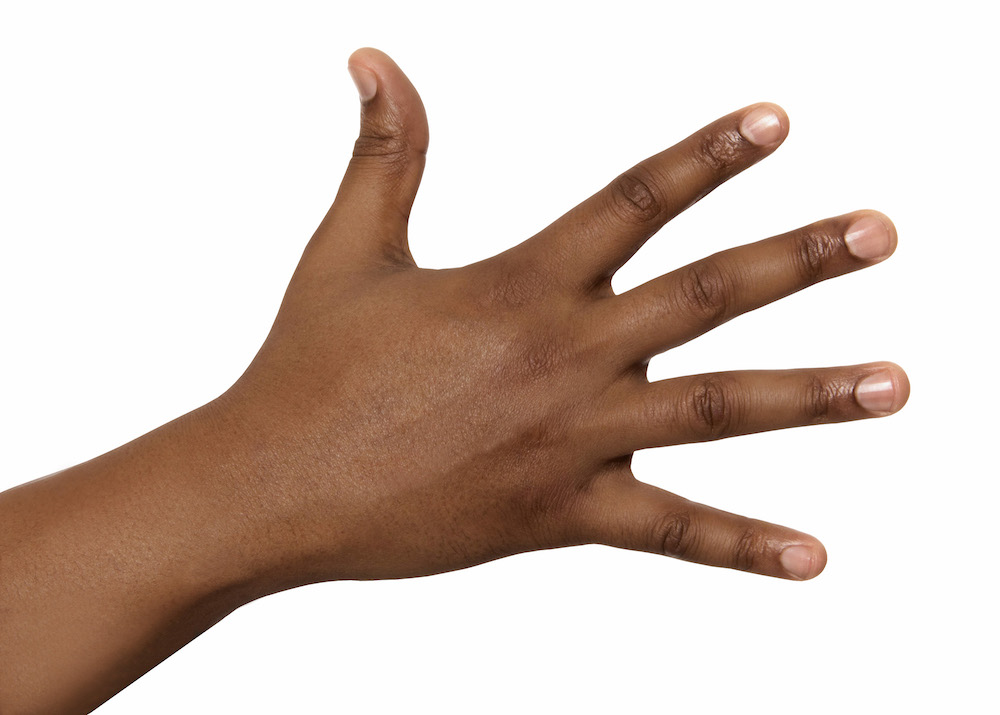
\includegraphics[width=\textwidth,height=\textheight,keepaspectratio]{../inputs/hand_dark.jpg}
  \end{minipage} & 
  \begin{minipage}{.29\textwidth}
    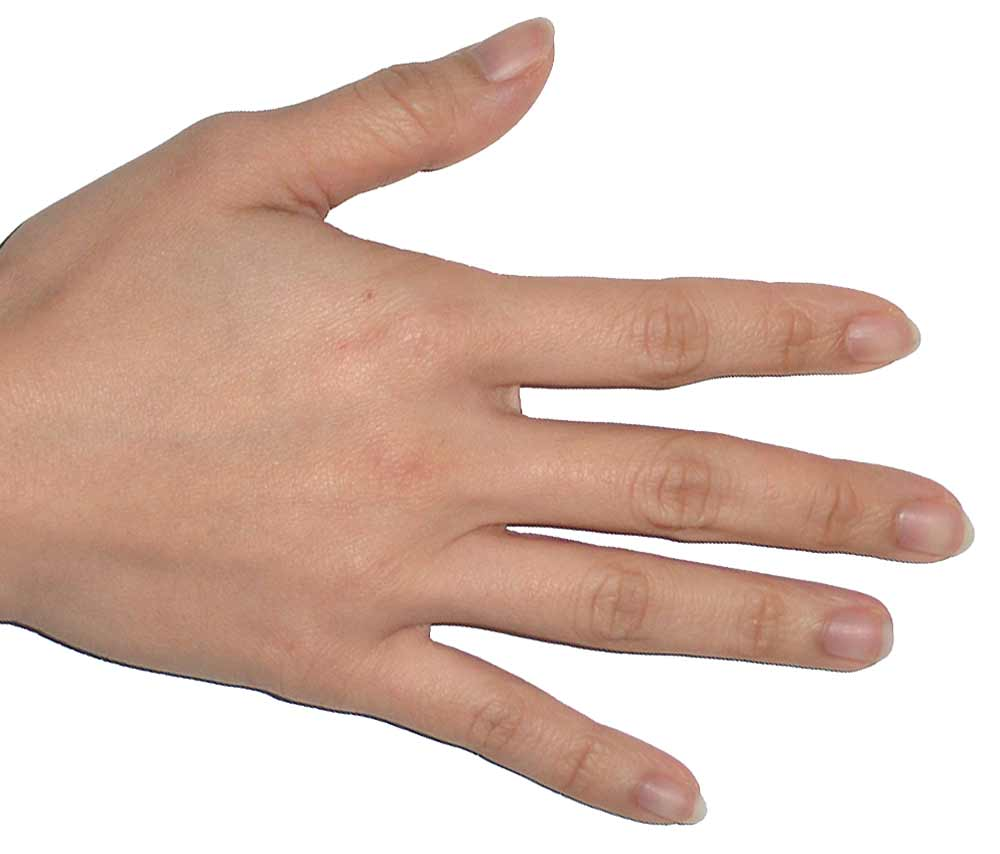
\includegraphics[width=\textwidth,height=\textheight,keepaspectratio]{../inputs/hand_light.jpg}
  \end{minipage} & 
  \begin{minipage}{.29\textwidth}
    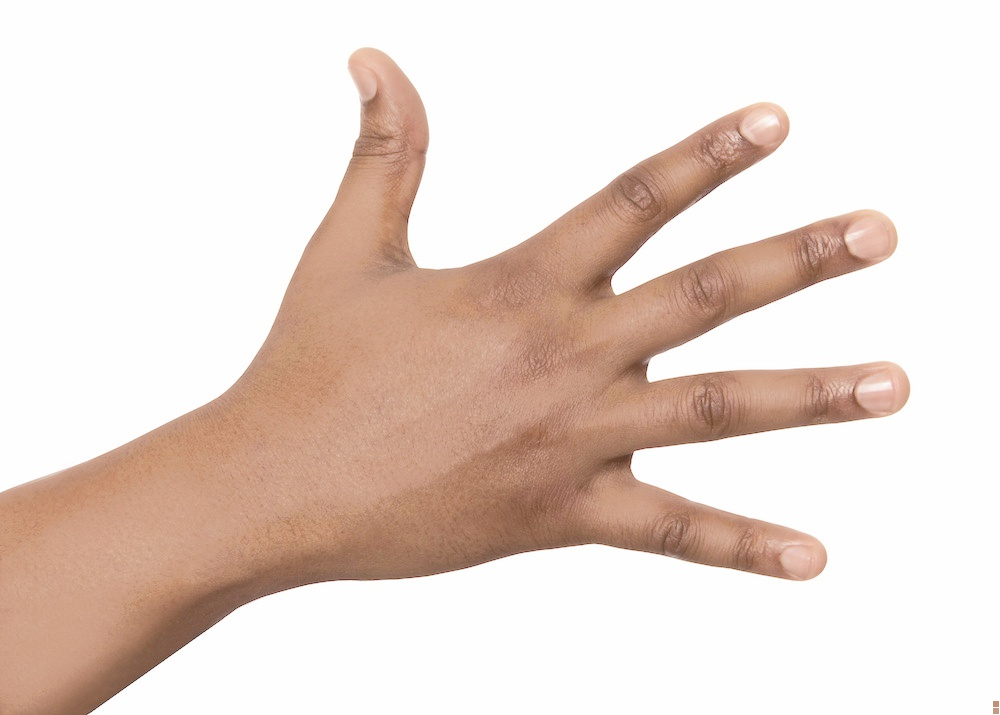
\includegraphics[width=\textwidth,height=\textheight,keepaspectratio]{../rc_test/outputs/20170521_proportional_corrected_test_alpha1p5/hand_dark_to_hand_light.jpg}
  \end{minipage} \\
\hline  \label{row:prop_correct_test_a1p5_hand_dark_to_hand_pale} &
  \begin{minipage}{.29\textwidth}
    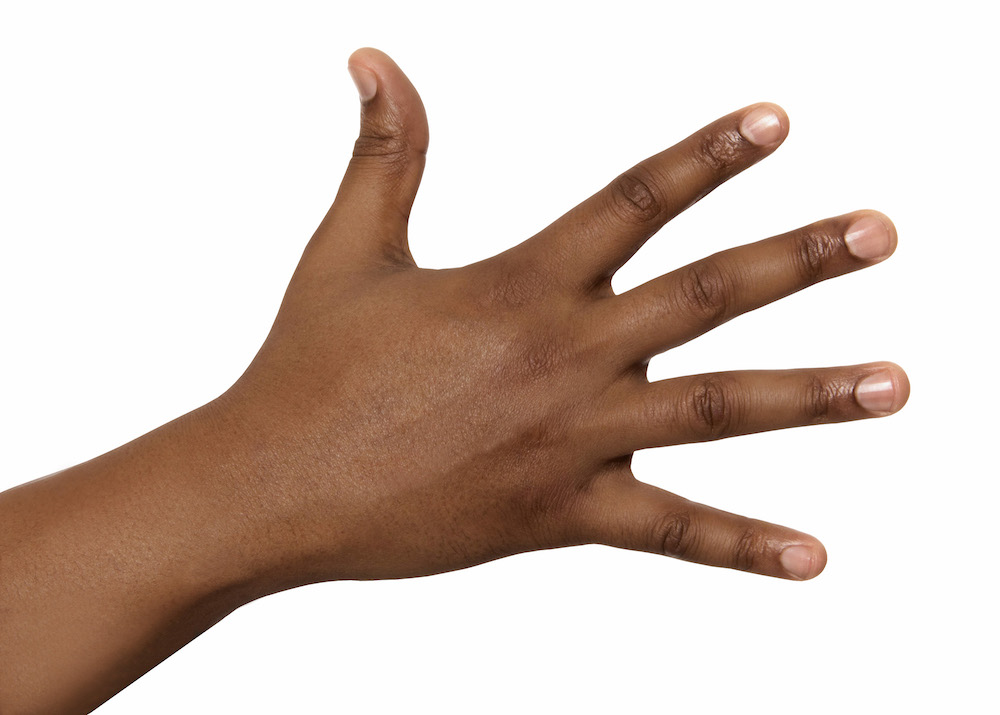
\includegraphics[width=\textwidth,height=\textheight,keepaspectratio]{../inputs/hand_dark.jpg}
  \end{minipage} & 
  \begin{minipage}{.29\textwidth}
    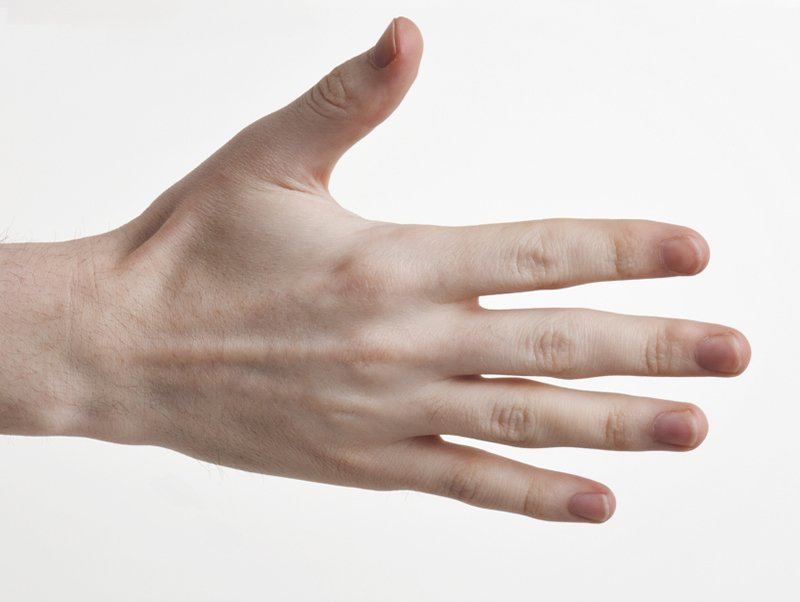
\includegraphics[width=\textwidth,height=\textheight,keepaspectratio]{../inputs/hand_pale.jpg}
  \end{minipage} & 
  \begin{minipage}{.29\textwidth}
    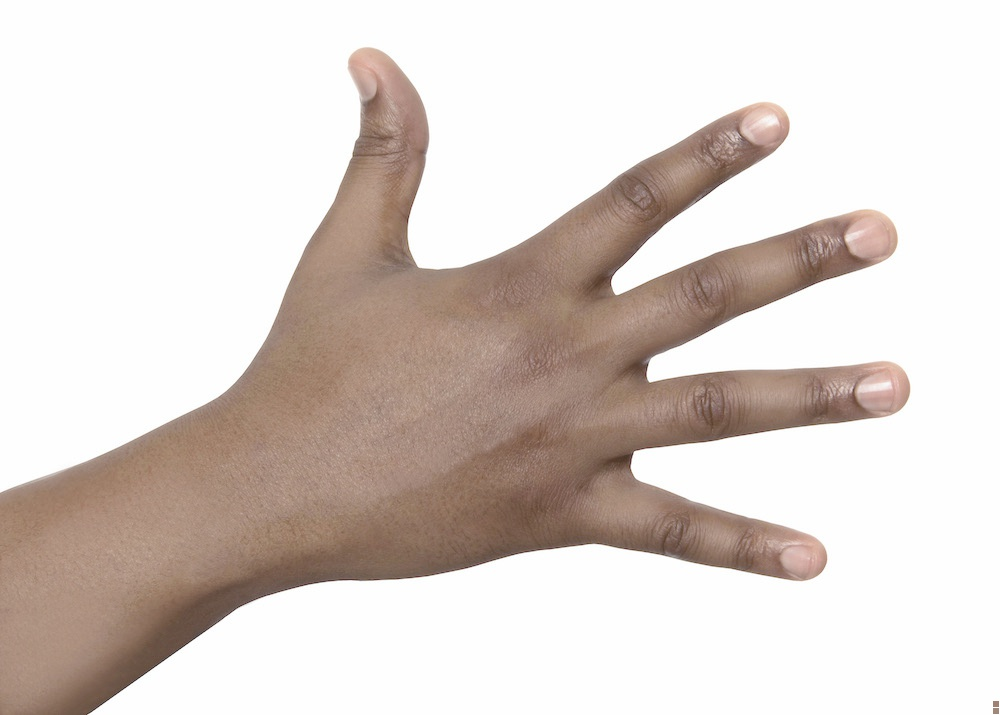
\includegraphics[width=\textwidth,height=\textheight,keepaspectratio]{../rc_test/outputs/20170521_proportional_corrected_test_alpha1p5/hand_dark_to_hand_pale.jpg}
  \end{minipage} \\
\hline  \label{row:prop_correct_test_a1p5_hand_brown_to_hand_dark} &
  \begin{minipage}{.29\textwidth}
    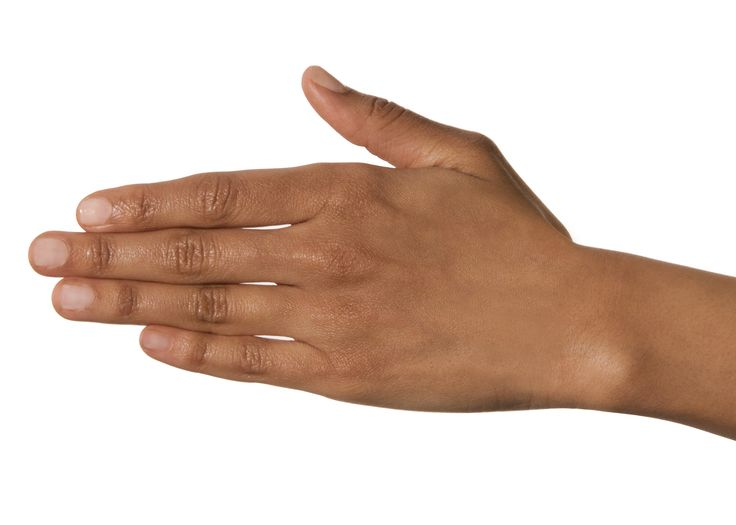
\includegraphics[width=\textwidth,height=\textheight,keepaspectratio]{../inputs/hand_brown.jpg}
  \end{minipage} & 
  \begin{minipage}{.29\textwidth}
    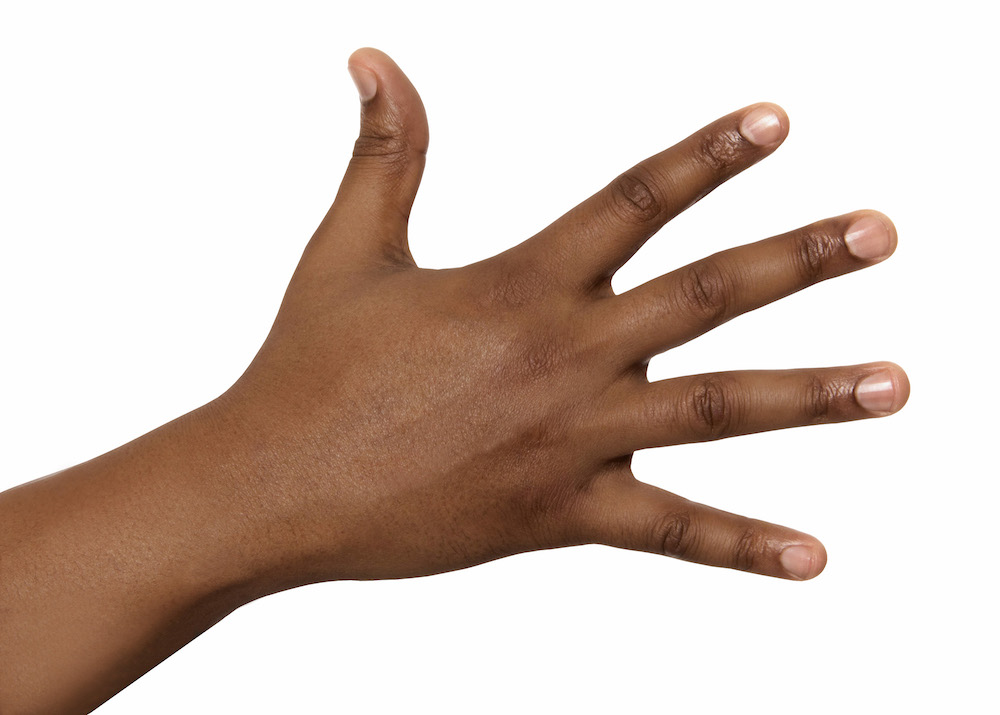
\includegraphics[width=\textwidth,height=\textheight,keepaspectratio]{../inputs/hand_dark.jpg}
  \end{minipage} & 
  \begin{minipage}{.29\textwidth}
    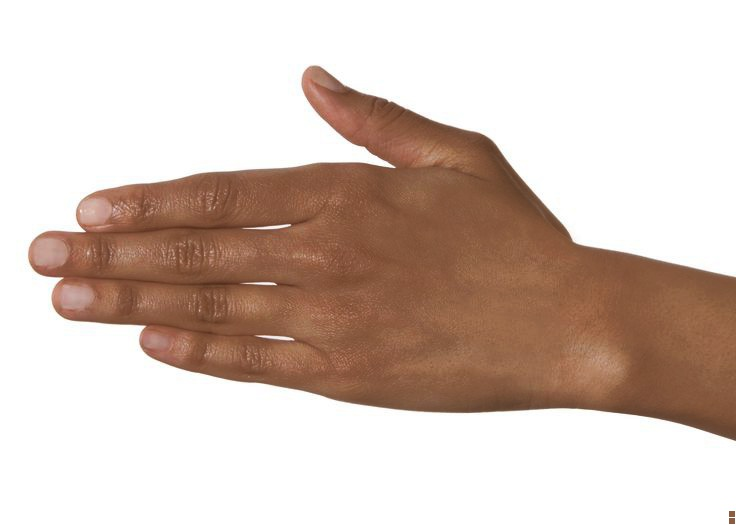
\includegraphics[width=\textwidth,height=\textheight,keepaspectratio]{../rc_test/outputs/20170521_proportional_corrected_test_alpha1p5/hand_brown_to_hand_dark.jpg}
  \end{minipage} \\
\hline  \label{row:prop_correct_test_a1p5_hand_brown_to_hand_light} &
  \begin{minipage}{.29\textwidth}
    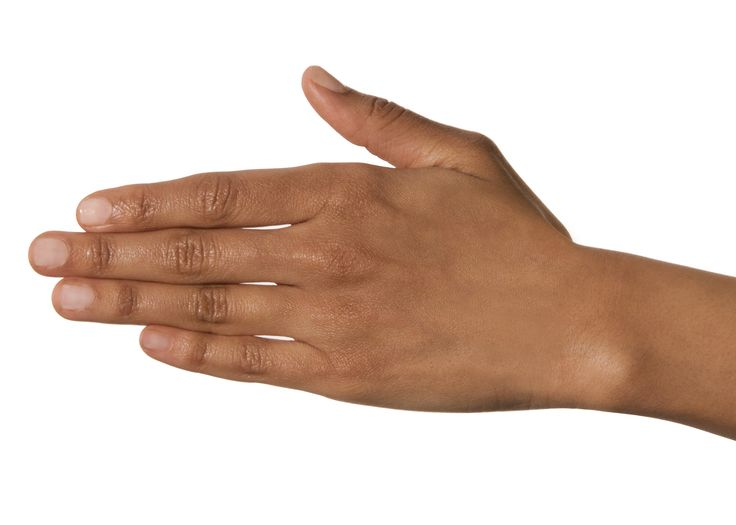
\includegraphics[width=\textwidth,height=\textheight,keepaspectratio]{../inputs/hand_brown.jpg}
  \end{minipage} & 
  \begin{minipage}{.29\textwidth}
    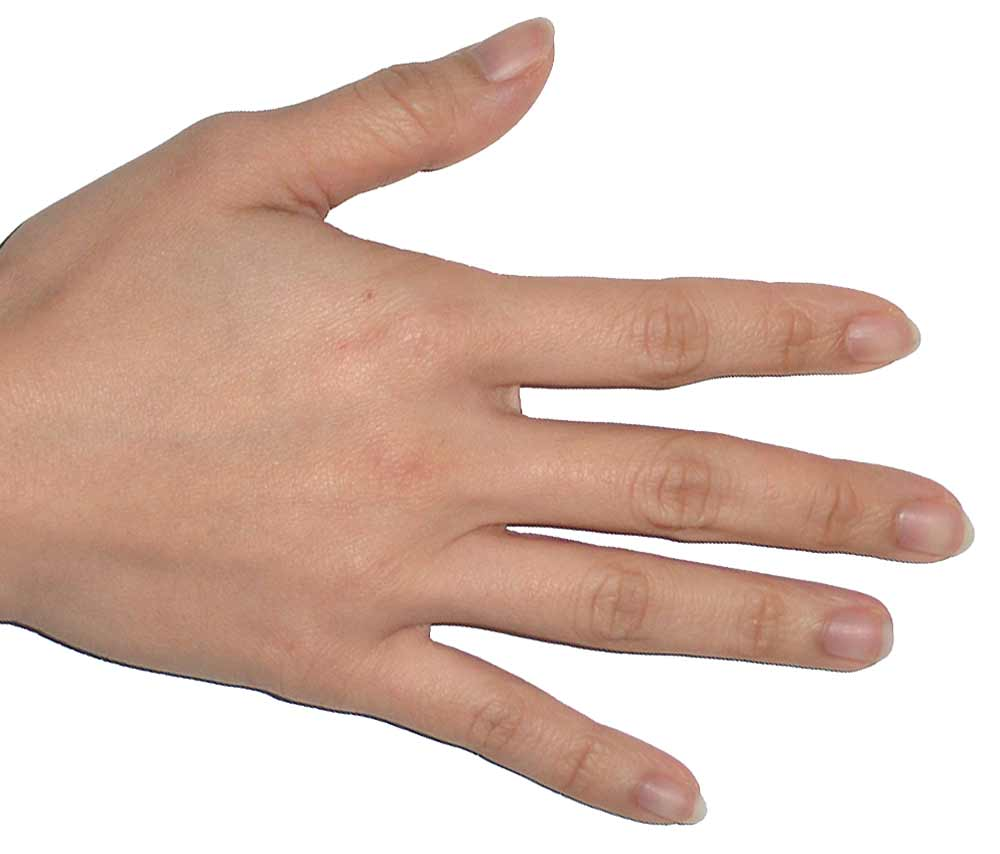
\includegraphics[width=\textwidth,height=\textheight,keepaspectratio]{../inputs/hand_light.jpg}
  \end{minipage} & 
  \begin{minipage}{.29\textwidth}
    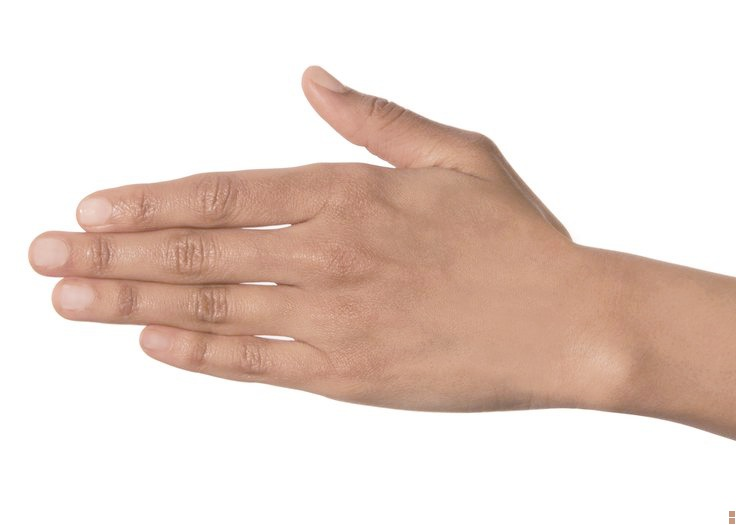
\includegraphics[width=\textwidth,height=\textheight,keepaspectratio]{../rc_test/outputs/20170521_proportional_corrected_test_alpha1p5/hand_brown_to_hand_light.jpg}
  \end{minipage} \\
\hline  \label{row:prop_correct_test_a1p5_hand_brown_to_hand_pale} &
  \begin{minipage}{.29\textwidth}
    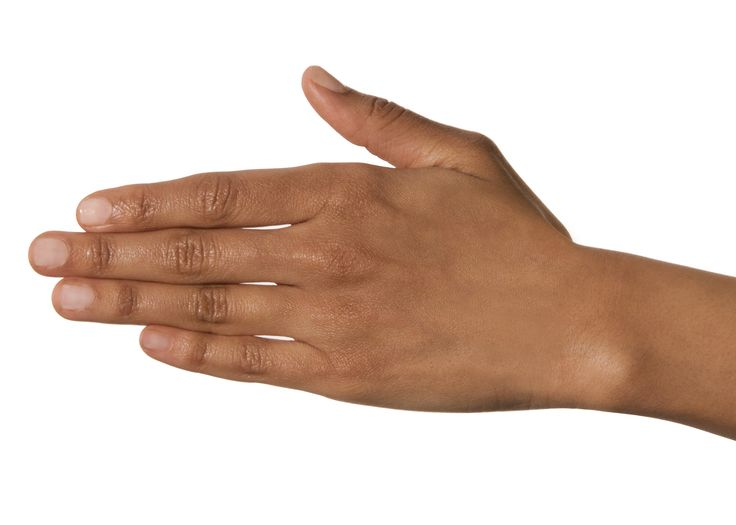
\includegraphics[width=\textwidth,height=\textheight,keepaspectratio]{../inputs/hand_brown.jpg}
  \end{minipage} & 
  \begin{minipage}{.29\textwidth}
    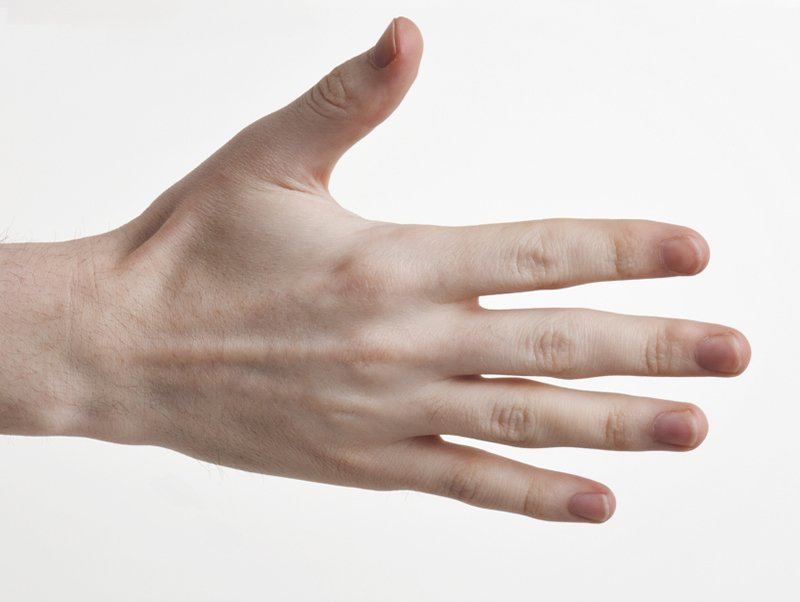
\includegraphics[width=\textwidth,height=\textheight,keepaspectratio]{../inputs/hand_pale.jpg}
  \end{minipage} & 
  \begin{minipage}{.29\textwidth}
    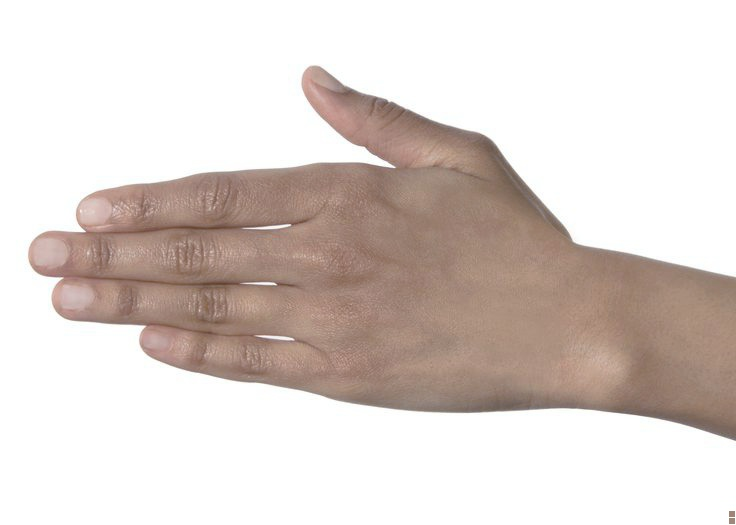
\includegraphics[width=\textwidth,height=\textheight,keepaspectratio]{../rc_test/outputs/20170521_proportional_corrected_test_alpha1p5/hand_brown_to_hand_pale.jpg}
  \end{minipage} \\
\hline  \label{row:prop_correct_test_a1p5_hand_light_to_hand_dark} &
  \begin{minipage}{.29\textwidth}
    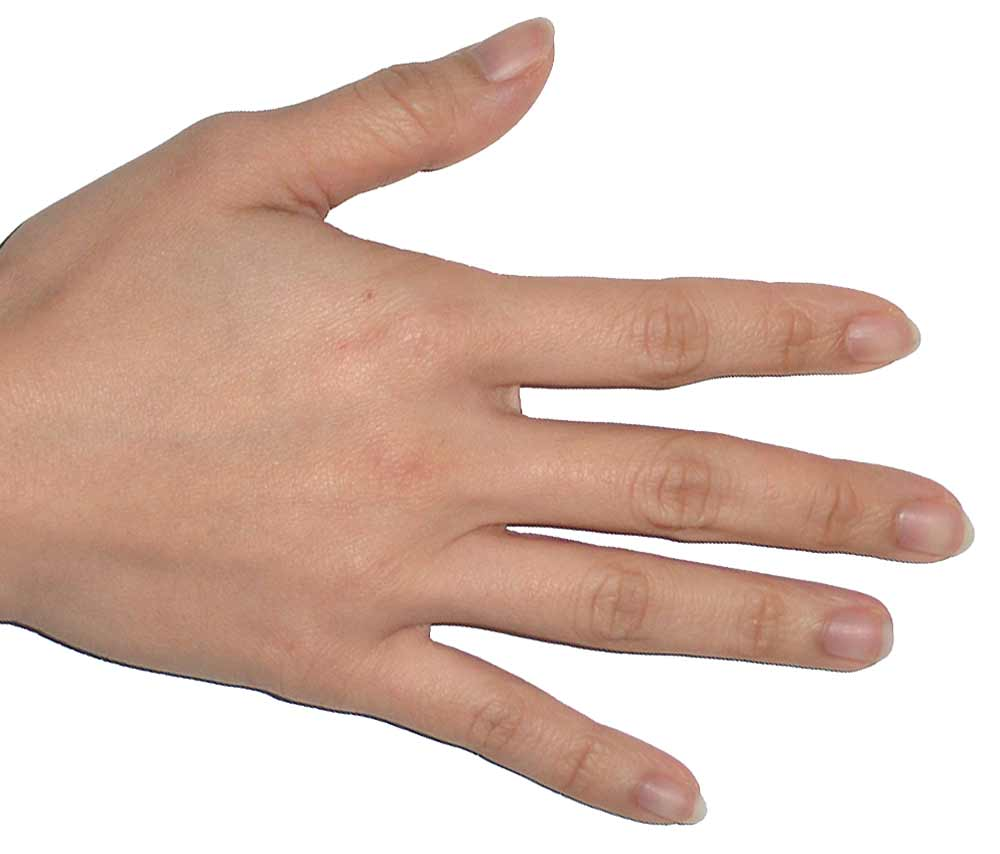
\includegraphics[width=\textwidth,height=\textheight,keepaspectratio]{../inputs/hand_light.jpg}
  \end{minipage} & 
  \begin{minipage}{.29\textwidth}
    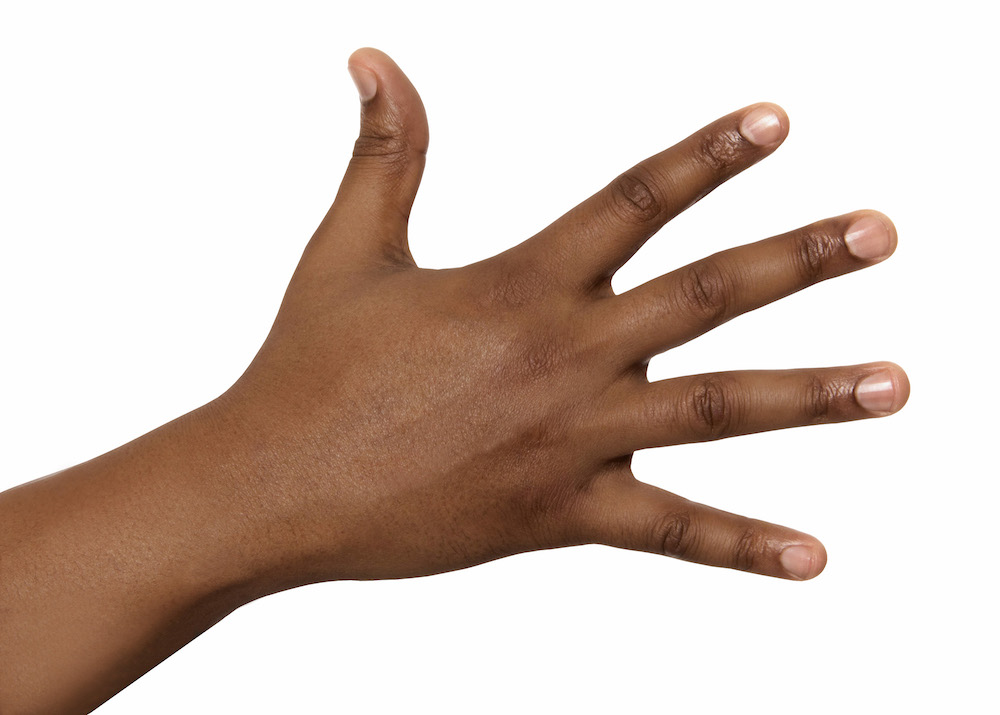
\includegraphics[width=\textwidth,height=\textheight,keepaspectratio]{../inputs/hand_dark.jpg}
  \end{minipage} & 
  \begin{minipage}{.29\textwidth}
    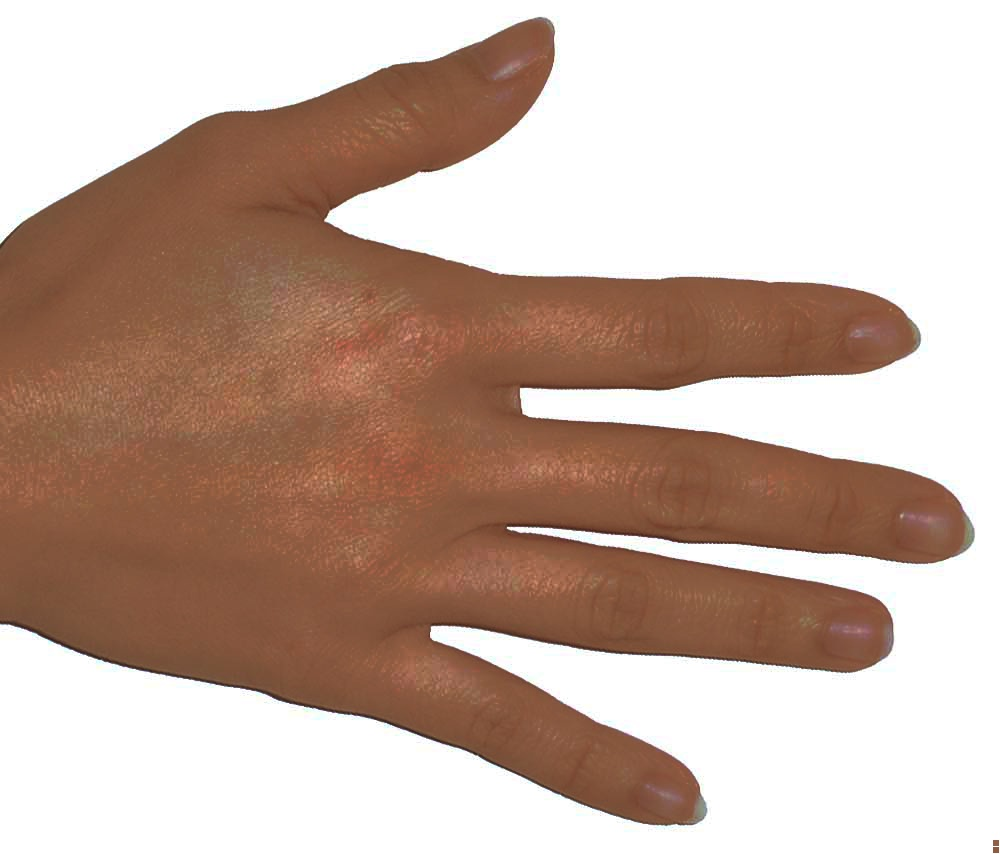
\includegraphics[width=\textwidth,height=\textheight,keepaspectratio]{../rc_test/outputs/20170521_proportional_corrected_test_alpha1p5/hand_light_to_hand_dark.jpg}
  \end{minipage} \\
\hline  \label{row:prop_correct_test_a1p5_hand_light_to_hand_brown} &
  \begin{minipage}{.29\textwidth}
    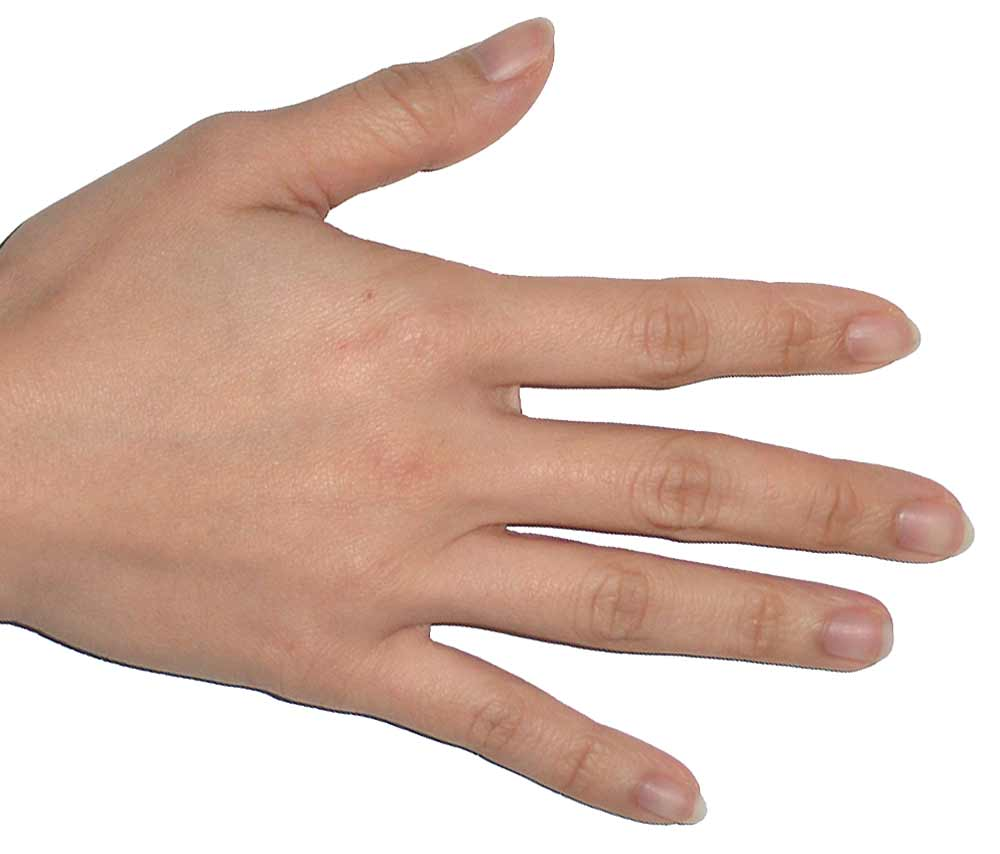
\includegraphics[width=\textwidth,height=\textheight,keepaspectratio]{../inputs/hand_light.jpg}
  \end{minipage} & 
  \begin{minipage}{.29\textwidth}
    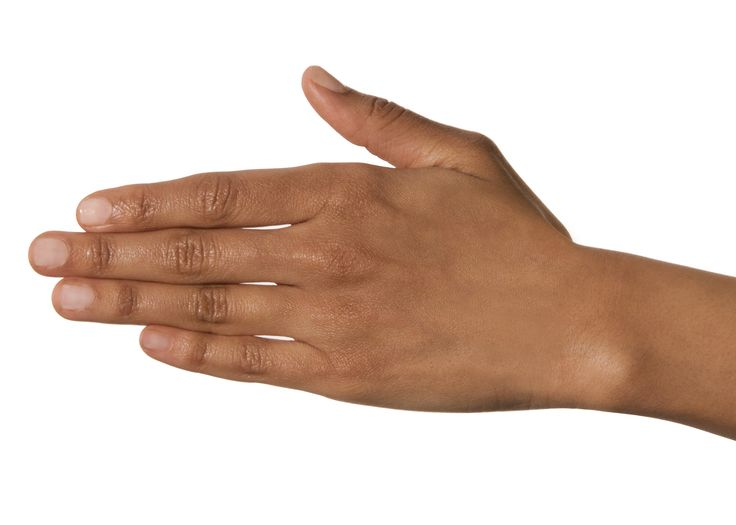
\includegraphics[width=\textwidth,height=\textheight,keepaspectratio]{../inputs/hand_brown.jpg}
  \end{minipage} & 
  \begin{minipage}{.29\textwidth}
    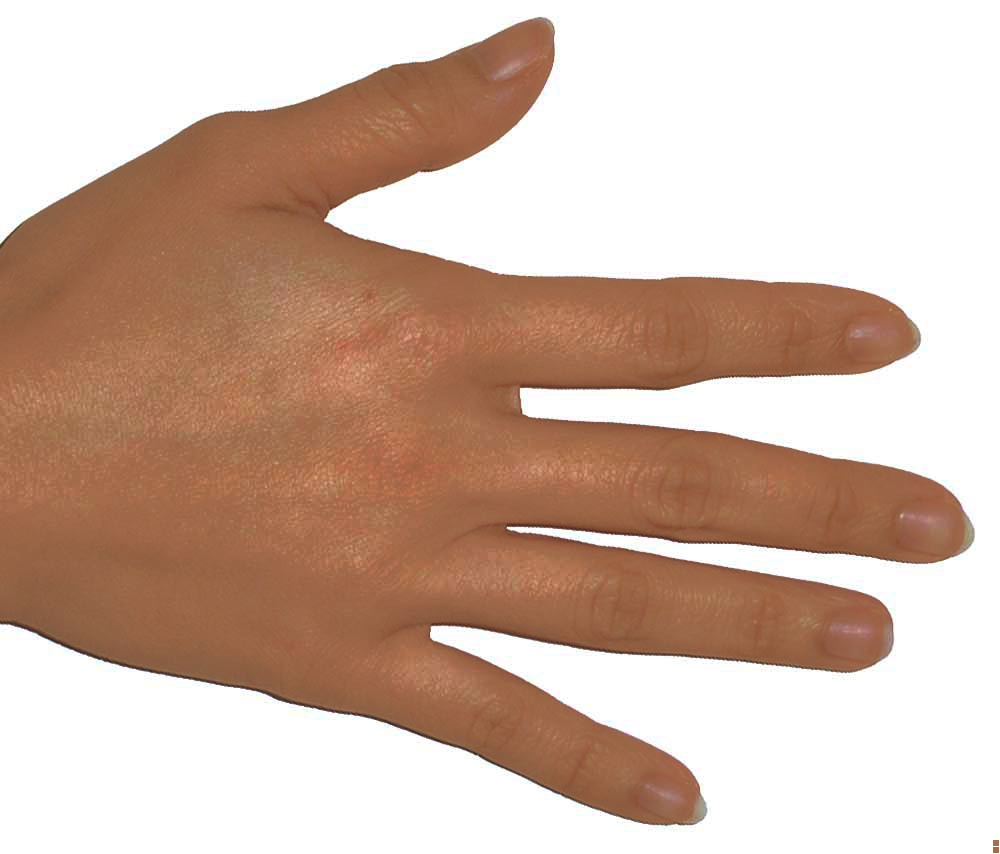
\includegraphics[width=\textwidth,height=\textheight,keepaspectratio]{../rc_test/outputs/20170521_proportional_corrected_test_alpha1p5/hand_light_to_hand_brown.jpg}
  \end{minipage} \\
\hline  \label{row:prop_correct_test_a1p5_hand_light_to_hand_pale} &
  \begin{minipage}{.29\textwidth}
    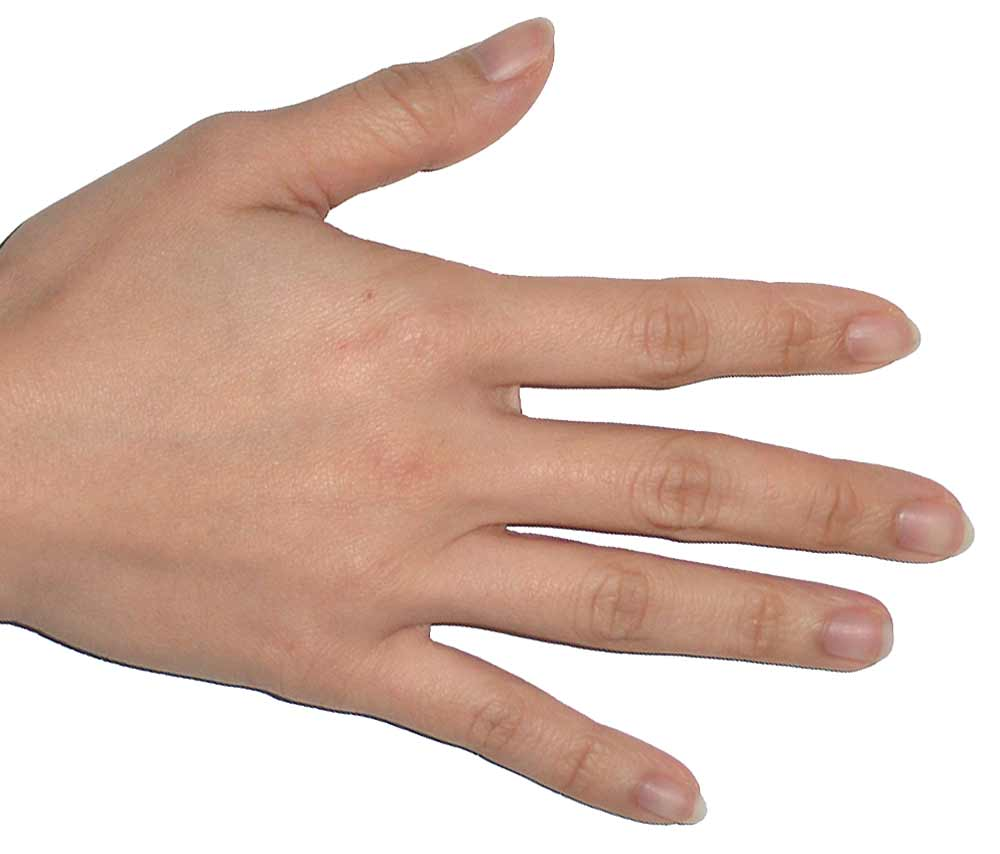
\includegraphics[width=\textwidth,height=\textheight,keepaspectratio]{../inputs/hand_light.jpg}
  \end{minipage} & 
  \begin{minipage}{.29\textwidth}
    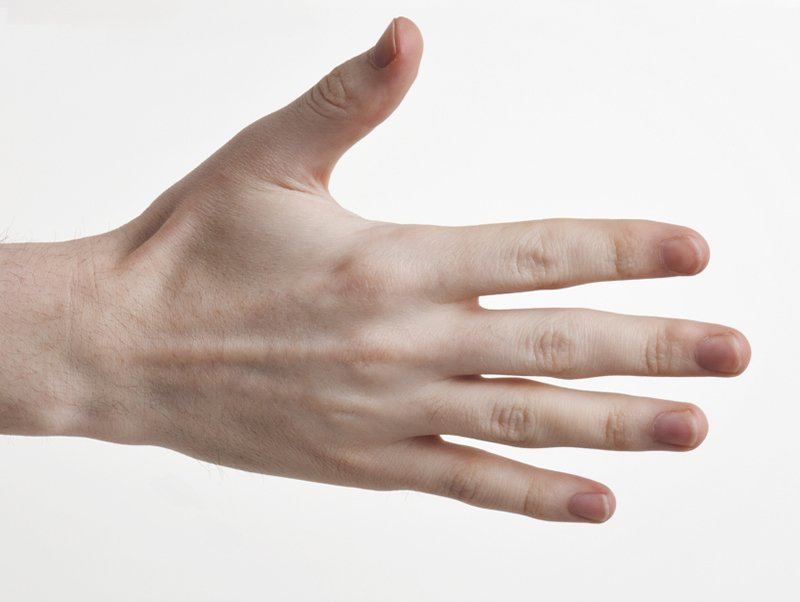
\includegraphics[width=\textwidth,height=\textheight,keepaspectratio]{../inputs/hand_pale.jpg}
  \end{minipage} & 
  \begin{minipage}{.29\textwidth}
    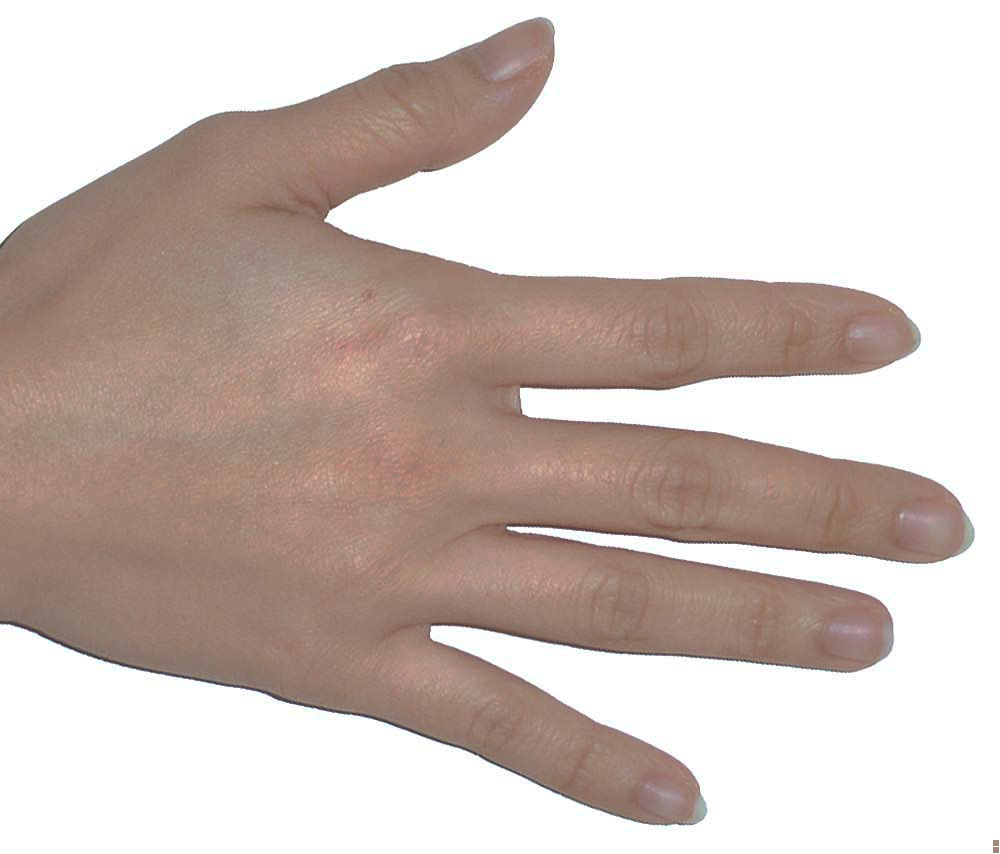
\includegraphics[width=\textwidth,height=\textheight,keepaspectratio]{../rc_test/outputs/20170521_proportional_corrected_test_alpha1p5/hand_light_to_hand_pale.jpg}
  \end{minipage} \\
\hline  \label{row:prop_correct_test_a1p5_hand_pale_to_hand_dark} &
  \begin{minipage}{.29\textwidth}
    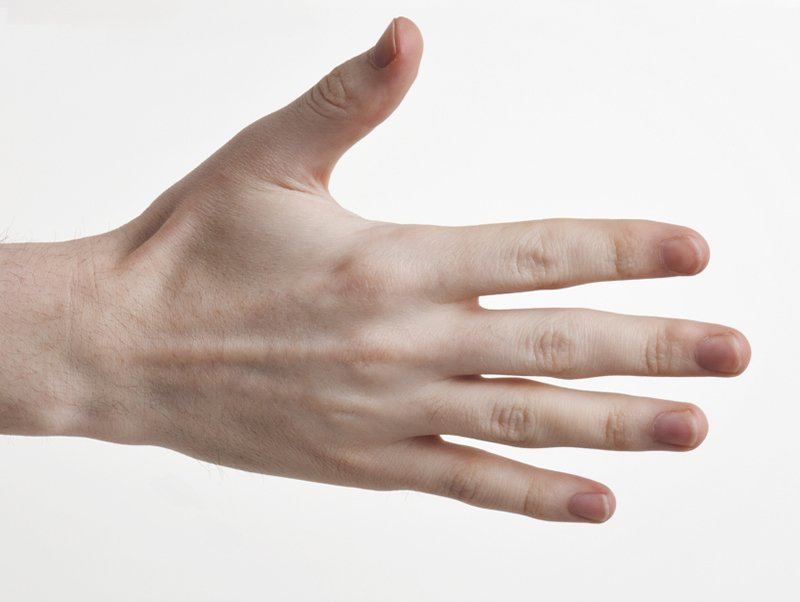
\includegraphics[width=\textwidth,height=\textheight,keepaspectratio]{../inputs/hand_pale.jpg}
  \end{minipage} & 
  \begin{minipage}{.29\textwidth}
    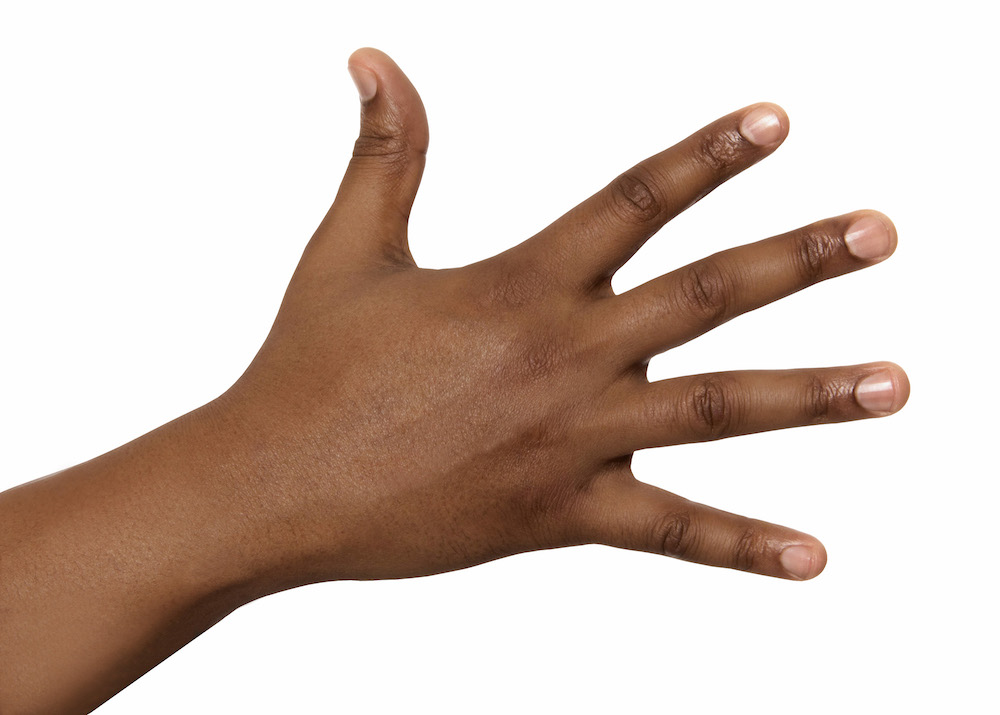
\includegraphics[width=\textwidth,height=\textheight,keepaspectratio]{../inputs/hand_dark.jpg}
  \end{minipage} & 
  \begin{minipage}{.29\textwidth}
    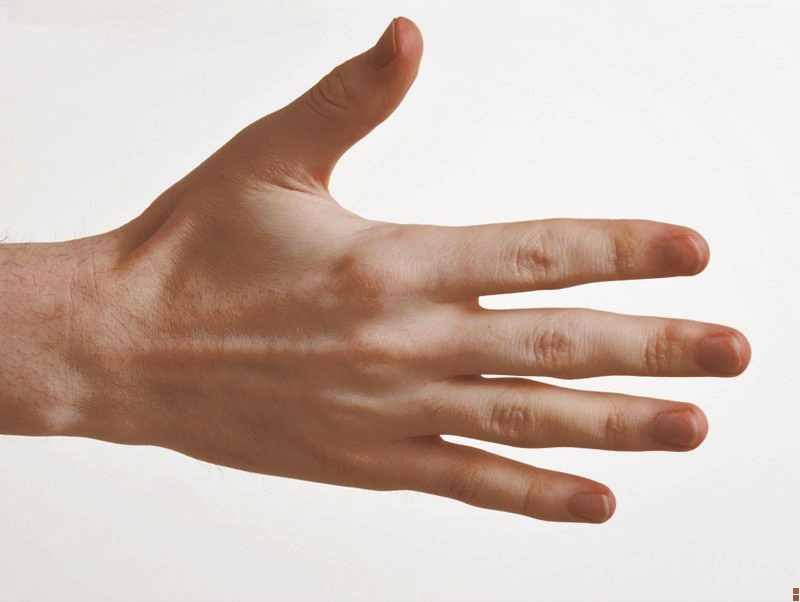
\includegraphics[width=\textwidth,height=\textheight,keepaspectratio]{../rc_test/outputs/20170521_proportional_corrected_test_alpha1p5/hand_pale_to_hand_dark.jpg}
  \end{minipage} \\
\hline  \label{row:prop_correct_test_a1p5_hand_pale_to_hand_brown} &
  \begin{minipage}{.29\textwidth}
    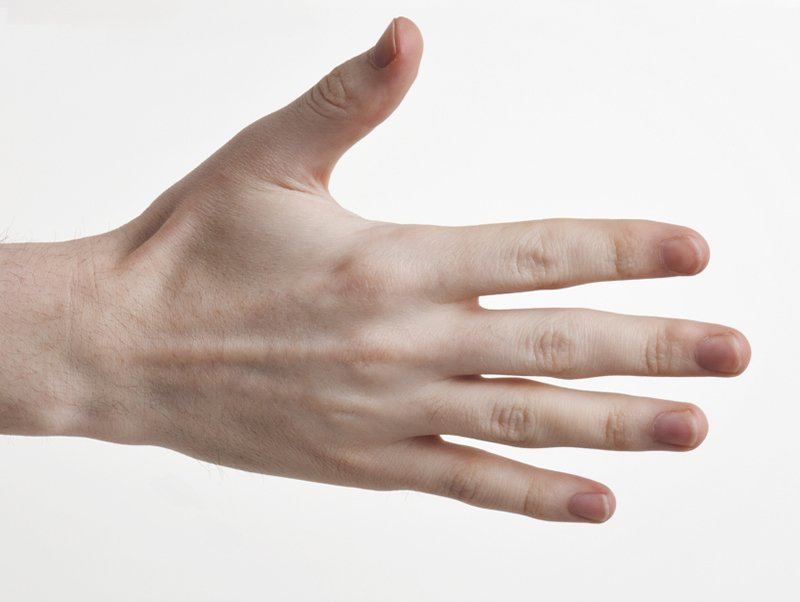
\includegraphics[width=\textwidth,height=\textheight,keepaspectratio]{../inputs/hand_pale.jpg}
  \end{minipage} & 
  \begin{minipage}{.29\textwidth}
    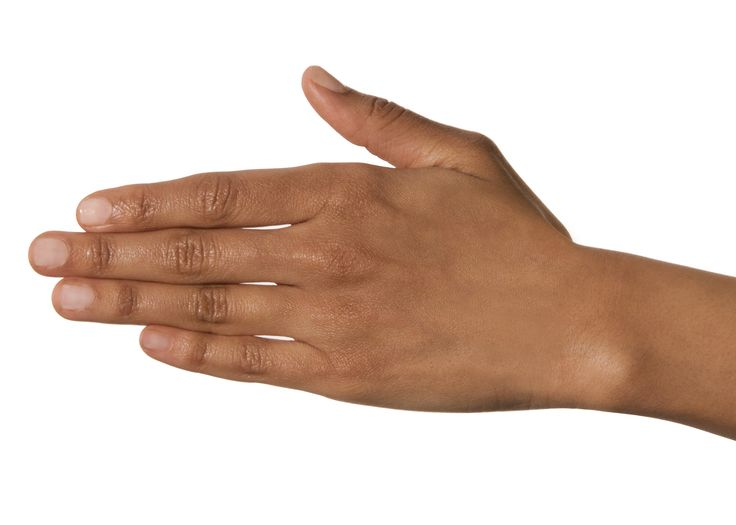
\includegraphics[width=\textwidth,height=\textheight,keepaspectratio]{../inputs/hand_brown.jpg}
  \end{minipage} & 
  \begin{minipage}{.29\textwidth}
    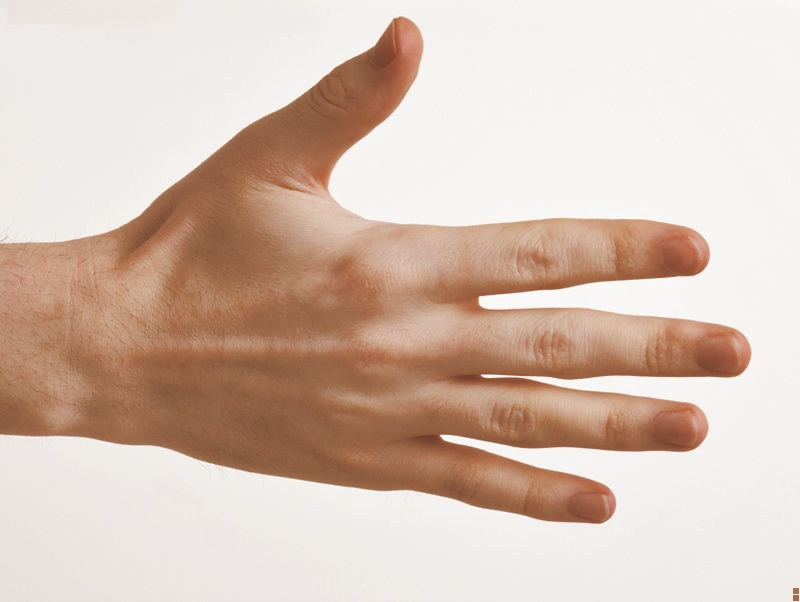
\includegraphics[width=\textwidth,height=\textheight,keepaspectratio]{../rc_test/outputs/20170521_proportional_corrected_test_alpha1p5/hand_pale_to_hand_brown.jpg}
  \end{minipage} \\
\hline  \label{row:prop_correct_test_a1p5_hand_pale_to_hand_light} &
  \begin{minipage}{.29\textwidth}
    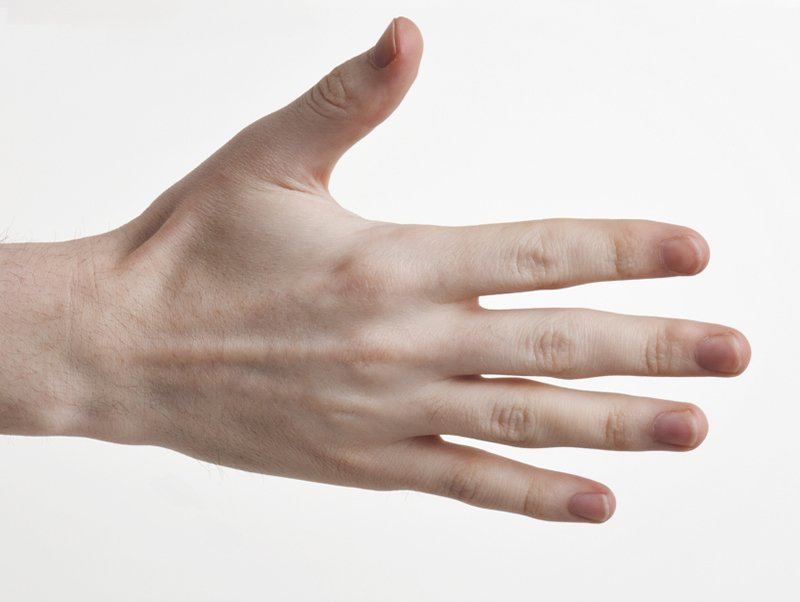
\includegraphics[width=\textwidth,height=\textheight,keepaspectratio]{../inputs/hand_pale.jpg}
  \end{minipage} & 
  \begin{minipage}{.29\textwidth}
    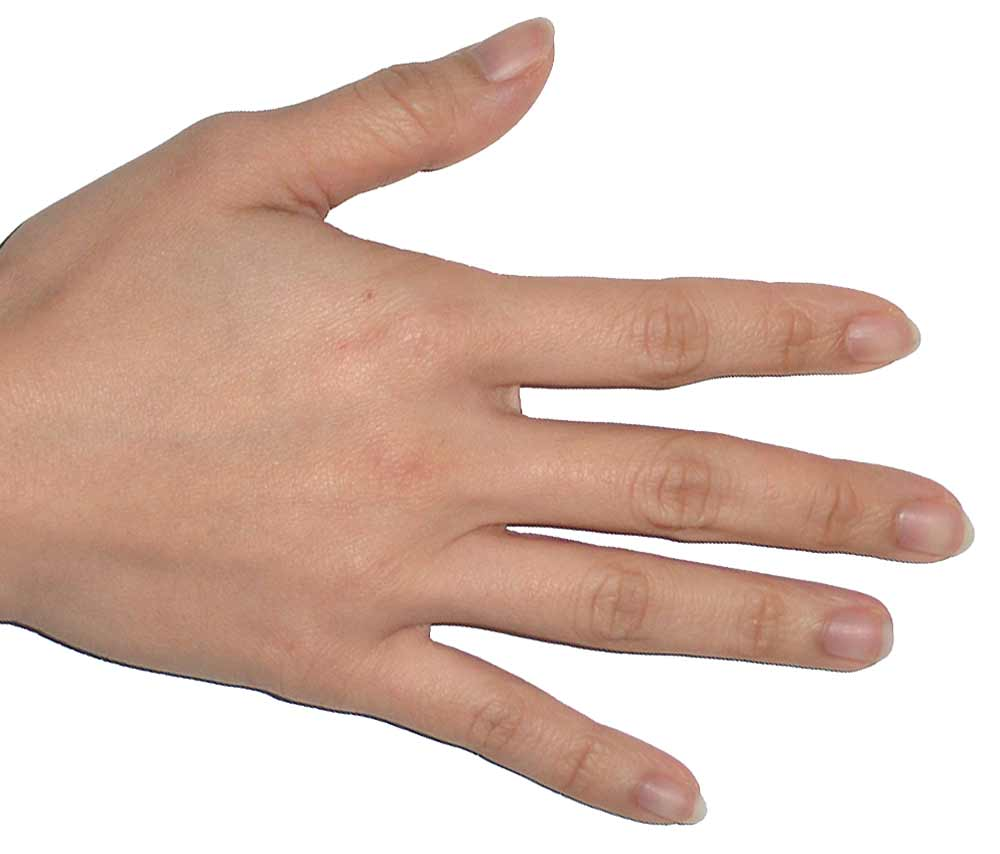
\includegraphics[width=\textwidth,height=\textheight,keepaspectratio]{../inputs/hand_light.jpg}
  \end{minipage} & 
  \begin{minipage}{.29\textwidth}
    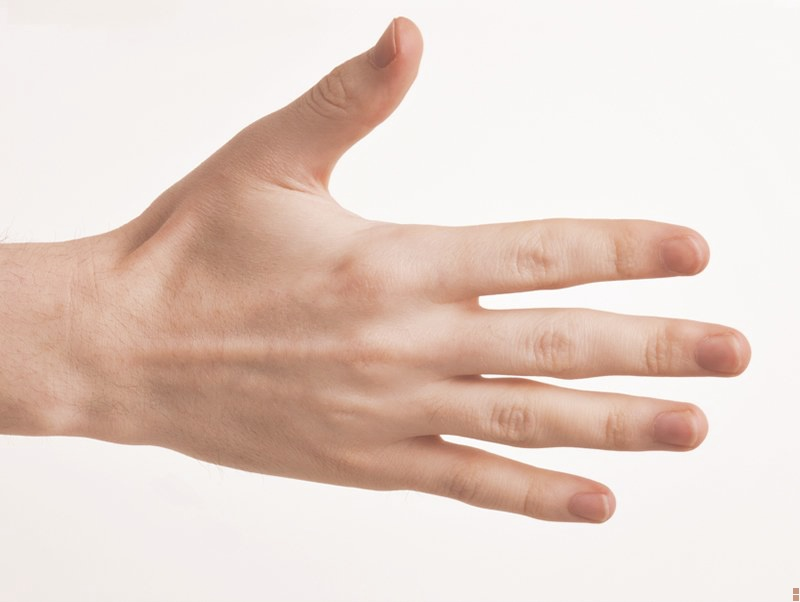
\includegraphics[width=\textwidth,height=\textheight,keepaspectratio]{../rc_test/outputs/20170521_proportional_corrected_test_alpha1p5/hand_pale_to_hand_light.jpg}
  \end{minipage} \\
\hline
 \end{longtable}

\end{document}